\chapter{Predicting the Future}

\section{Idea}

The first policy we look at is formerly called Multi-Level Feedback Queue or MLFQ short. The create Fernando J. Corbató recieved a Turning Award for it in 1990. 
As the title already says, this policy tries to predict the future behaviour of the processes based on the past.
A job can be generally act in two ways.
Either it is a resources intensive crunching problem (think about exporting a video or compiling code) or it is a program, which needs quick response time (think about your text editor).
In reality most jobs jump between these two states.
We usually want to give the response based processes priority, because that is what the user interacts with and it is here that he primarily feels a delay.

The policy is based on multiple queues, which have each different priorities.
Each process gets assigned to a queue. There are however not set in stone
Based on the reasons above we want to assume that a new process is responsive, because in the worst case scenario, we need to just demote the non-responsive ones.
If however a process turns out to be interactive, than the user does not feel any lag. 
Each process can run a certain amount of time (also called allotment time) before it is deemed as unworthy of the current priority.
If the allotment is used up the process get demoted into a queue below.

\begin{figure}[h]
    \centering
    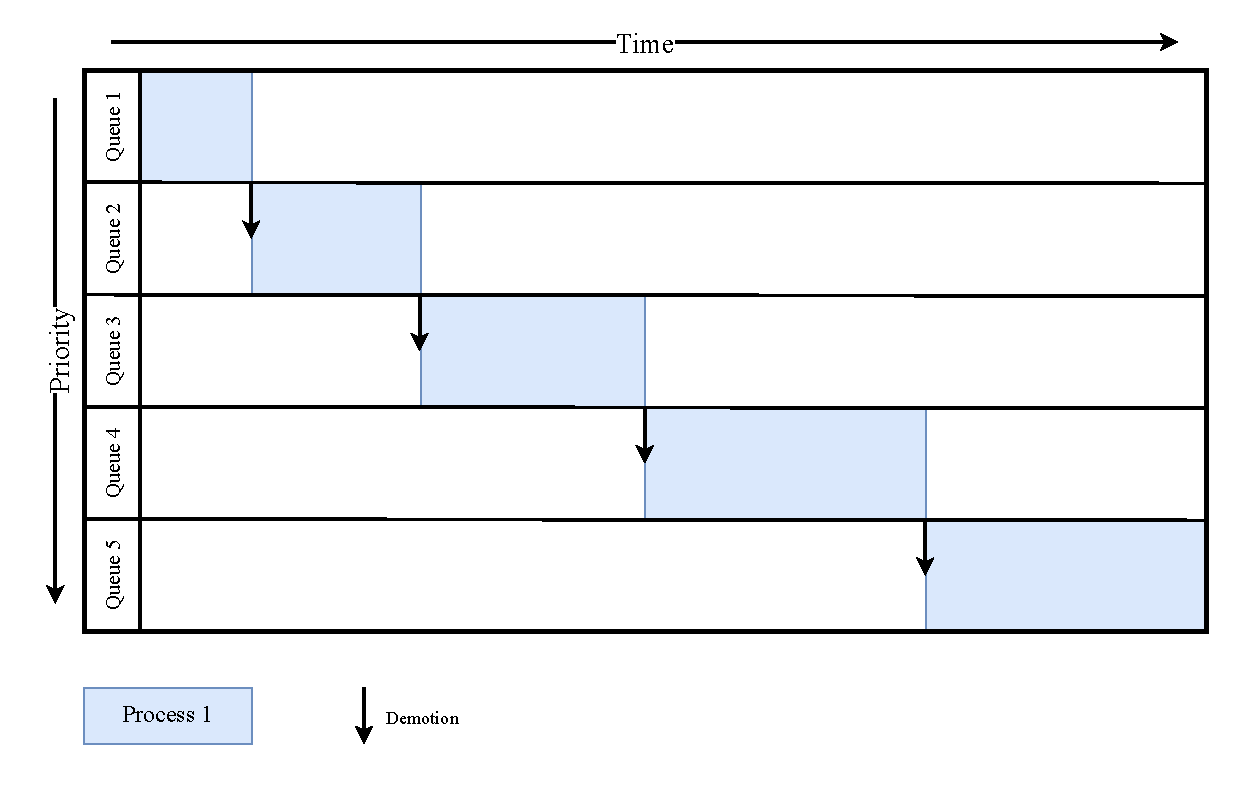
\includegraphics[width=0.7\textwidth]{Assets/MLFQ-Example-1.pdf}
    \caption{Simple working of MLFQ}
    \label{fig:mlfq-example-1}
\end{figure}


As you can see in figure \ref{fig:mlfq-example-1} the process one gets demoted after a while.
Also the lower the queue is, the higher the allotment time. 
This is because we hope that all of the responsive focused finish before demoting.
Once these are filtered out we have only resource heavy tasks left.
These require more time anyways, so the allotment time is stretched out.

\section{Multiple Processes}

What happens if we introduce another process?
Well, it depends on the priorities. 
Higher priority recieves the CPU time.
If they are on the same queue, than they run using Round Robin, see section \ref{sec:rr}.


\begin{figure}[h]
    \centering
    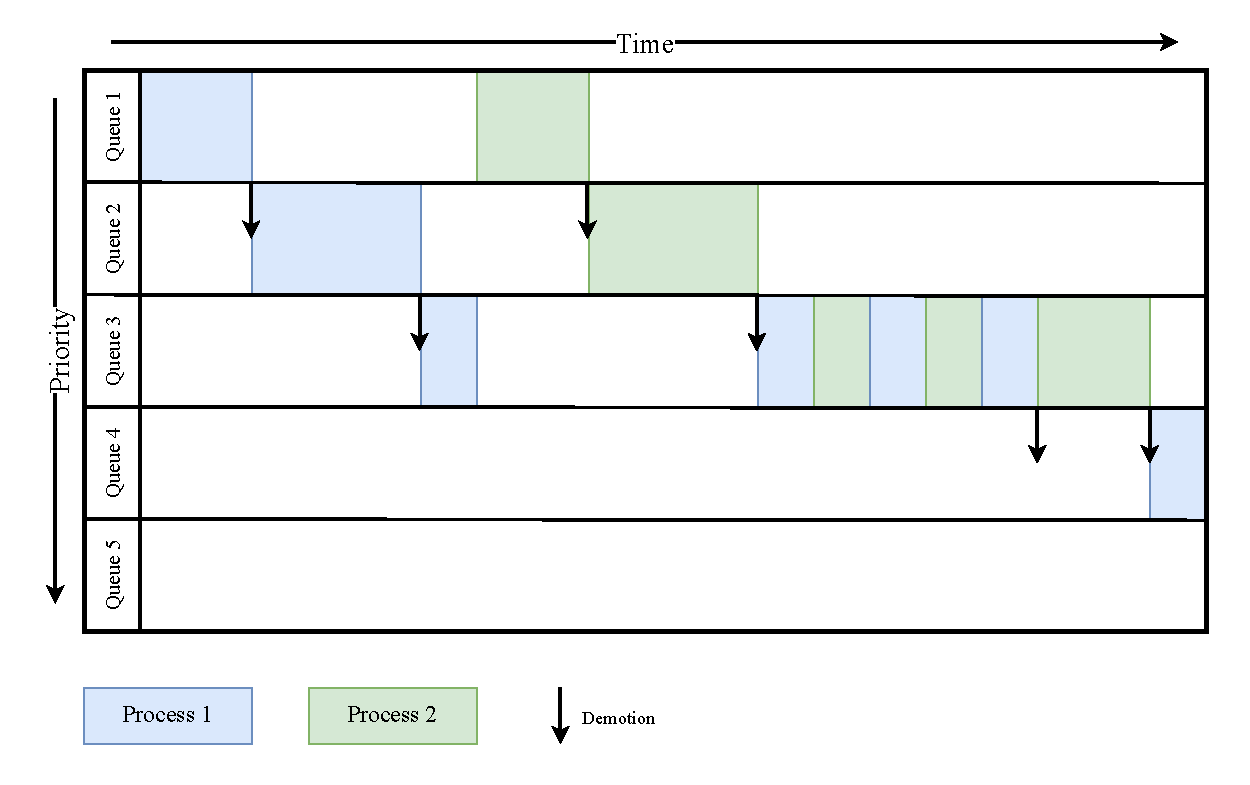
\includegraphics[width=0.7\textwidth]{Assets/MLFQ-Example-2.pdf}
    \caption{Running multiple processes in MLFQ}
    \label{fig:mlfq-example-2}
\end{figure}

As you can see in figure \ref{fig:mlfq-example-2} once process two is introduced process one is temporarily starved. The problem is solved once they land on the same queue.
There they run alternately.
Still the more tasks we introduce the more prevalent the starving issue gets.

\begin{figure}[h]
    \centering
    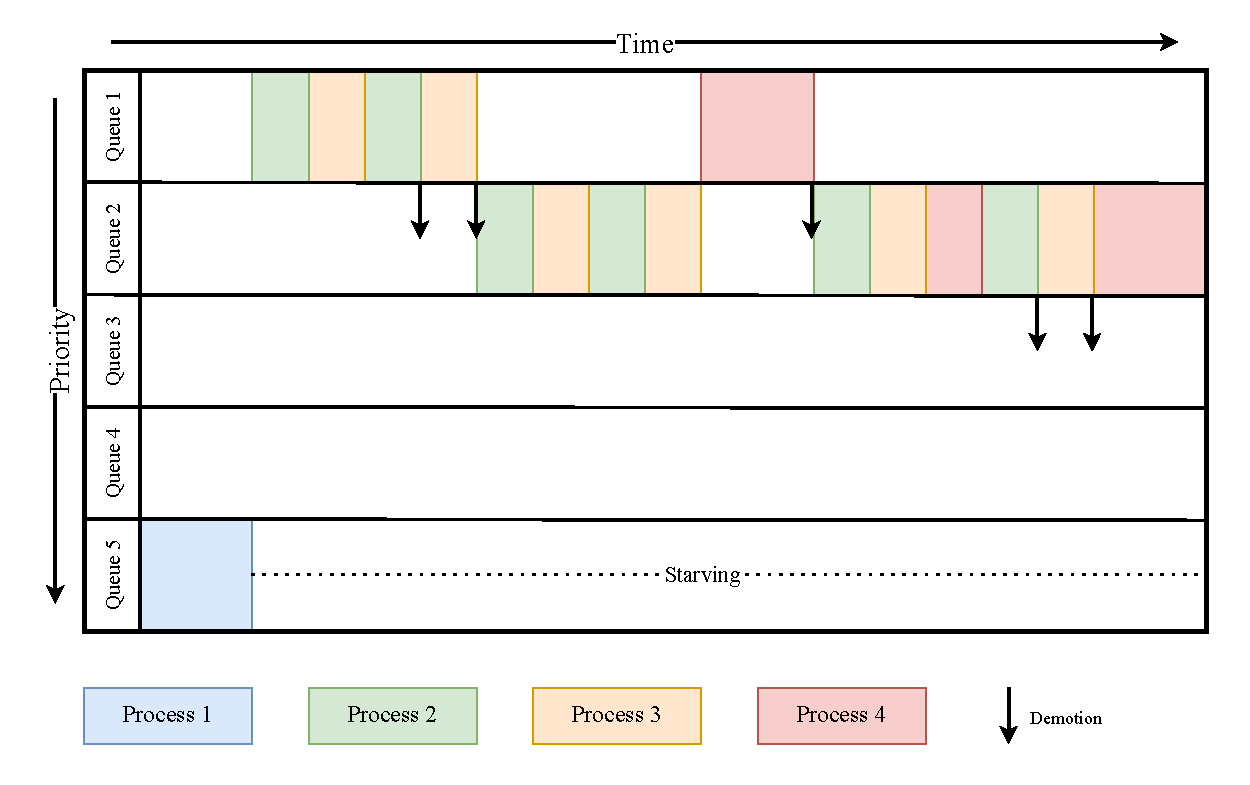
\includegraphics[width=0.7\textwidth]{Assets/MLFQ-Example-3.pdf}
    \caption{Starving Processes in MLFQ}
    \label{fig:mlfq-example-3}
\end{figure}

\section{Solving the Starving Problem}

Solving starvation is actually easy.
All we have to make sure that once in a while everybody gets their deserved CPU time.
To do that we introduce a priority boost. All it does is just put every process into priority one every so often.

\begin{figure}[h]
    \centering
    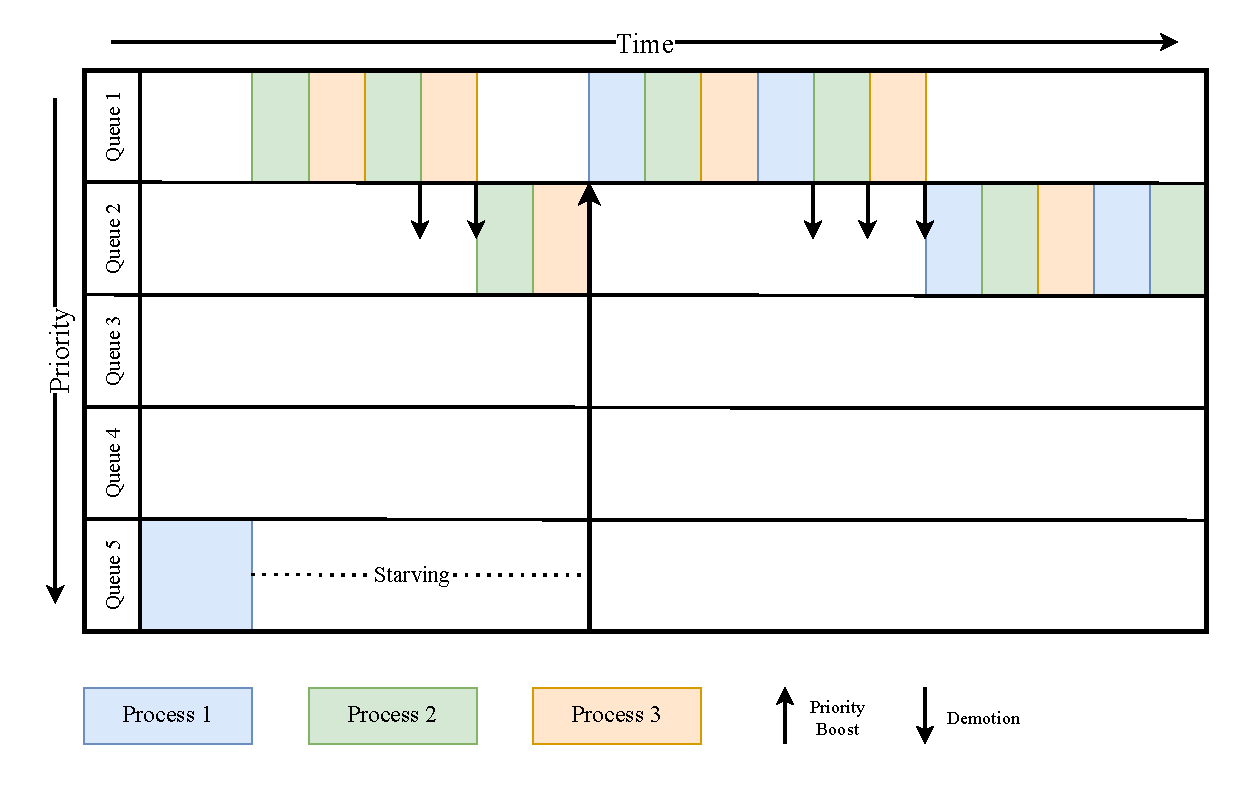
\includegraphics[width=0.7\textwidth]{Assets/MLFQ-Example-4.pdf}
    \caption{Solving Starvation in MLFQ}
    \label{fig:mlfq-example-4}
\end{figure}

\section{Wrapping Up}

This chapter showed us, how one could approach a scheduling policy that works without needing to know the burst time.
In the end we still end up with many variable like the allotment time per queue, the amount of queues, the quanta for the Round Robin and others.
If used in a real system the best approach would be to set some sensible defaults and let the administrator to adjust the parameters when needed.

\chapter{Scheduling Based on Tickets}

\section{How do tickets work?}

Tickets are a form of currency for the computer.
These can be handed out by the scheduler and give a process the right to use a resource.
Usually this is done proportianally to the amount of tickets.
Meaning a higher share of tickets will lead to a higher amount of CPU time.
Logically the response time is reverse proportional.
These tickets enable easy comparison between processes and their resources.
One important difference between a currency in real life and tickets is that tickets are consumed when used.
Practically this means that if you buy something you won't lose your bill.
This property leads to the tickets representing the share of the CPU that the job has.

\section{Operating with Tickets}

You can do two notable things with tickets. First you can transfer them. 
This does exactly what it means. You decrease your amount of tickets and increase someone else's. 
With this you could temporarily boost other processes.
Say, for example, you have a server and a client.
If the client needs something from the server, than it could temporarily boost the servers resources by transfering some of his own tickets.
If course this would require that the server is trusted or else it could just scam you out of your tickets.
The second way to operate with tickets is ticket inflation and deflation. This can only be done by the owner of the currency and it is only something that we will look at the next section.

\section{Ticket Currencies}

Ticket currencies are a way for parent processes to manage their child processes.
Yes, that's right, not all processes are built the same.
A child process is a process that is created by another process.
A parent process is a process, which has atleast one child process.
A job can be both at the same time.

The idea behind ticket currencies is that a parent process creates its own unique currency. Therefore he himself can distribute as many bills as he wants. 
However more custom bills does not equal to a higher share of CPU time in the whole system.
Take figure \ref{fig:ticket-currencies} for example. Even though process A had created 100 tickets and gave 40 to process A$_1$ in the end it is all about ratios.
Therefore the overall runtime that A$_1$ has is: 

$$\frac{20\text{T}_\text{G}}{50\text{T}_\text{G}} * \frac{40\text{T}_\text{A}}{100\text{T}_\text{A}} = 0.16 \Rightarrow 16\%$$

There is another hidden benefit. If the parent process recieves more global tickets, than if it has a custom currency, there are no further things to do.
If however it does not have a custom currency than the process has to transfer these new tickets to the child processes. Overall it can get very messy all too quickly.

\begin{figure}[h]
    \centering
    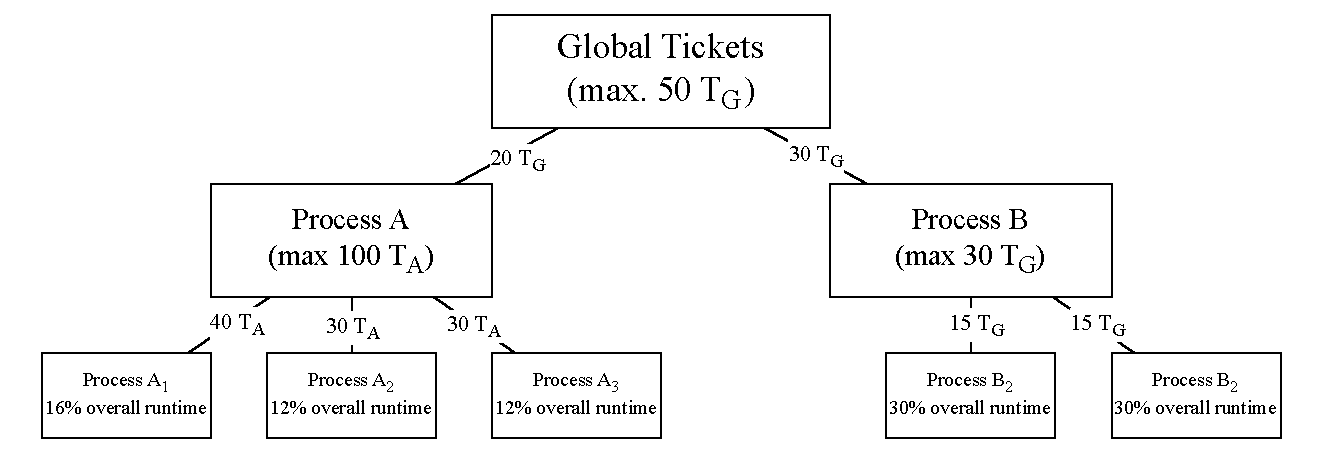
\includegraphics[width=\textwidth]{Assets/Ticket-Currency.pdf}
    \caption{Example of a Custom Ticket Currency}
    \label{fig:ticket-currencies}
\end{figure}
 
Another benefit comes with custom currencies: the ticket inflation or deflation operation.
One needs a custom currency, because it involves creating or destroying tickets. 
Still unlike the ticket transfer, ticket inflation does not need a sender and reciever.
The selected process just get more tickets assigned.
With this the parent process changes the ration of ownership and therefore boosts the selected job.


\section{Lottery Scheduling}

Like other things in computer science the name already says a lot. 
Here randomization is exploited to achieve the proportianal share in runtime.
The concept that if even over a small scale there will be unavoidable errors, the longer the scheduler runs the more accurate the share becomes.
Think of the tickets as lottery tickets.
If the randomization is fair, than the more tickets you have the more you will win.
There is a downside though.
The randomizer algorithm can get pretty expensive.
There is a way to reuse one random seed though, but we will only quickly touch upon it later.

For an example implementation in C take a look at figure \ref{code:lottery-sched}
This is taken from phd-mit-tr677.pdf (CITATION)

\begin{figure}[h]
    \begin{minted}[mathescape,
        linenos,
        numbersep=5pt,
        gobble=2,
        frame=lines,
        framesep=2mm,
        ]{cpp}
  /* Implementation of List-Based Lottery Scheduling Algorithm (Written by: pdh-mit-tr667.pdf CITATION) */

  /*per-client state */
  typedef struct {
    ...
    int tickets;
  } *client_t;

  /* current resource owner */
  client_t current;

  /* list of clients competing for resource */
  list_t list;

  /*global tick et sum */
  int global_tickets= 0;

  /* initialize client withspecified allocation */
  void client_init(client_t c, int tickets)
  {
    /*initialize client state, updateglobal sum */
    c->tickets = tickets;
    global_tickets += tickets;
    /*join competition for resource */
    list_insert(list, c);
  }

  void allocate()
  {
    int winner, sum;
    client_t c;
    /* randomly select winning tick et */
    winner = fast_random() % global_tickets;
    /* searchlist to find client with winning tick et */
    sum = 0;
    for (c = list_first(list);
         c != NULL;
         c = list_next(list, c))
    {
        /*update running sum, stop at winner */
        sum += c->tickets;
        if (sum > winner)
            break;
    }
    /*grant resource to winner forquantum */
    current = c;
    use_resource(current);
  }
    \end{minted}
    \label{code:lottery-sched}
    \caption{C: Lottery Scheduling}
\end{figure}


One could also use Binary trees...